\chapter{Discussion}
 \label{sec:discussion}

The experiments show that synthetic augmentation can slightly improve Raman-based glioma classification. However, they also reveal a substantial domain gap between generated and real spectra, especially in the 6-class grading task.

Combining synthetic and real spectra in the TSR/TR setting generally improved downstream classification performance across multiple models. This showcases the potential of synthetic spectra to improve the generalization capabilities of downstream models used in small-cohort settings. Therefore, instead of relying on synthetic spectra as a complete replacement for real measurements, they might be of greater use as a regularization strategy. 

To characterize the relationship between the real and synthetic spectral distributions beyond aggregate classification metrics, we examined two complementary embedding methods: PCA and $t$-SNE. Both were computed on $z$-scored, pooled real and synthetic spectra (up to $2000$ spectra per class per source). $t$-SNE was applied to the top $50$ principal components due to the high dimensionality ($N_\lambda$) of the input space. Each embedding is displayed twice: coloured by source (real vs.\ synthetic) and by diagnostic class (IDH-Mutant vs.\ IDH-Wildtype). The results are shown in Figure~\ref{fig:pca_tsne}.

\begin{figure}[h]
    \centering
    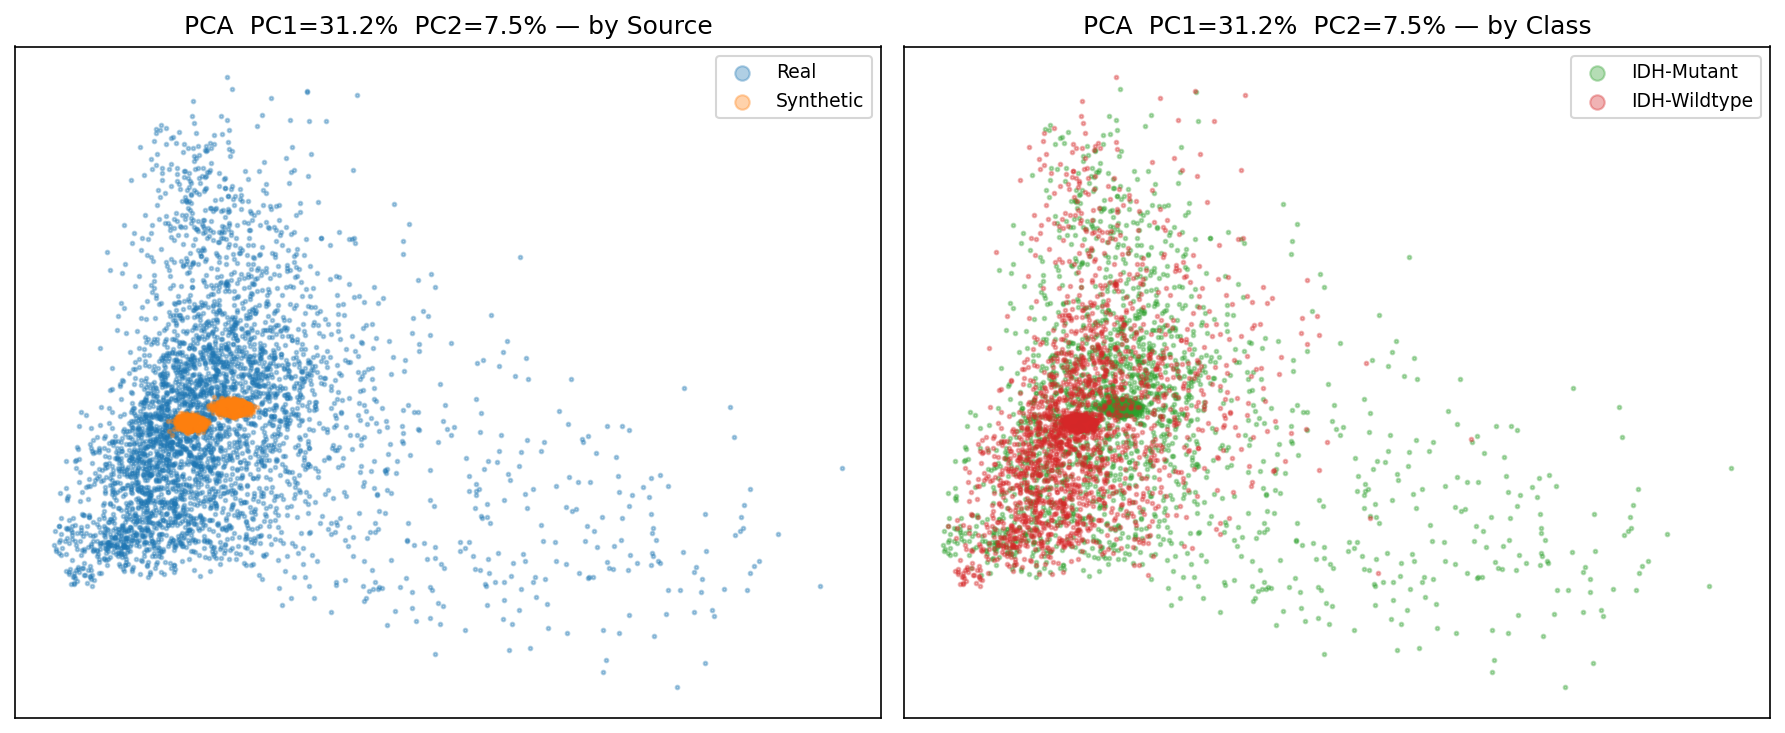
\includegraphics[width=\textwidth]{images/PCA.png}\\[4pt]
    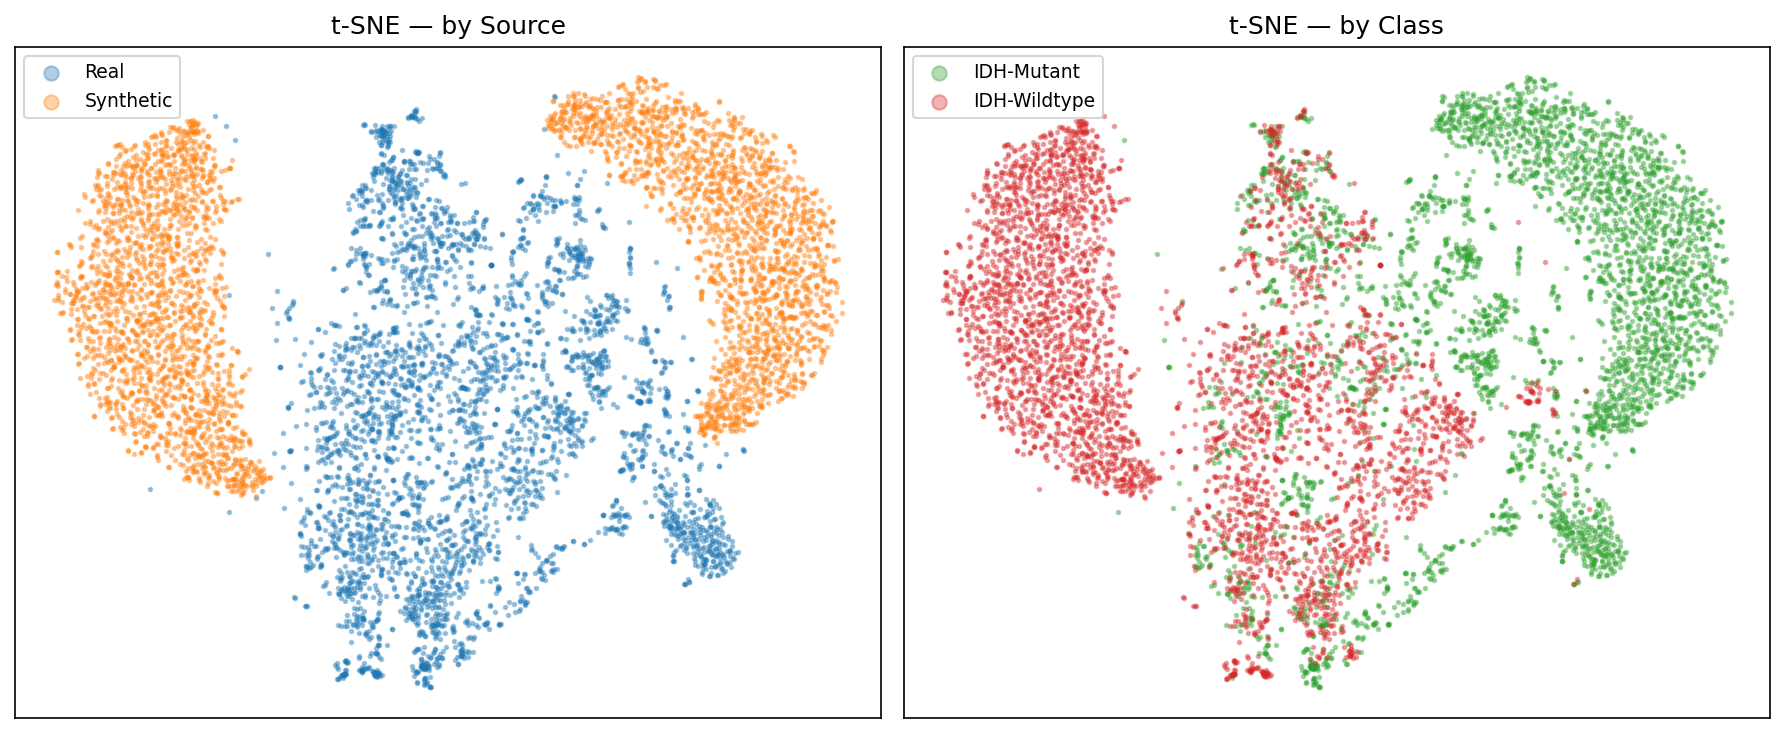
\includegraphics[width=\textwidth]{images/TSNE.png}
    \caption{\footnotesize PCA (top) and $t-$SNE (bottom) embeddings of real and synthetic spectra, coloured by source (left) and class (right).}
    \label{fig:pca_tsne}
\end{figure}

Taken together, the PCA and t-SNE plots offer insight into the spatial structure of the spectral data. The PCA plots reveal a variance difference between the real and the synthetic data sets: synthetic data forms two distinct clusters (corresponding to the two classes) with low variance, while the real data shows higher variance, and the two classes overlap to a great extent. Correlating these plots with the t-SNE plots, we can see that synthetic data is structured in two distinct clusters, whereas the raw data has a heterogeneous structure. It is worth noting that both the PCA and the t-SNE plots show the real data being intertwined. We hypothesize that the two classes might overlap (in the initial space) to such an extent that, under a strict, slide-isolated experiment, the possible accuracy for this particular dataset has a definite upper bound. 

We can visualize the spectral variance by plotting the mean spectrum of the real data and that of the synthetic data along with their standard deviation ($\sigma$) envelopes. We observe that the synthetic data standard deviation is much narrower than that of the real data, which suggests that the synthetic data is generally very close to the mean spectrum (Fig. \ref{fig:mean_std_spectra}).

\begin{figure}[h]
\centering
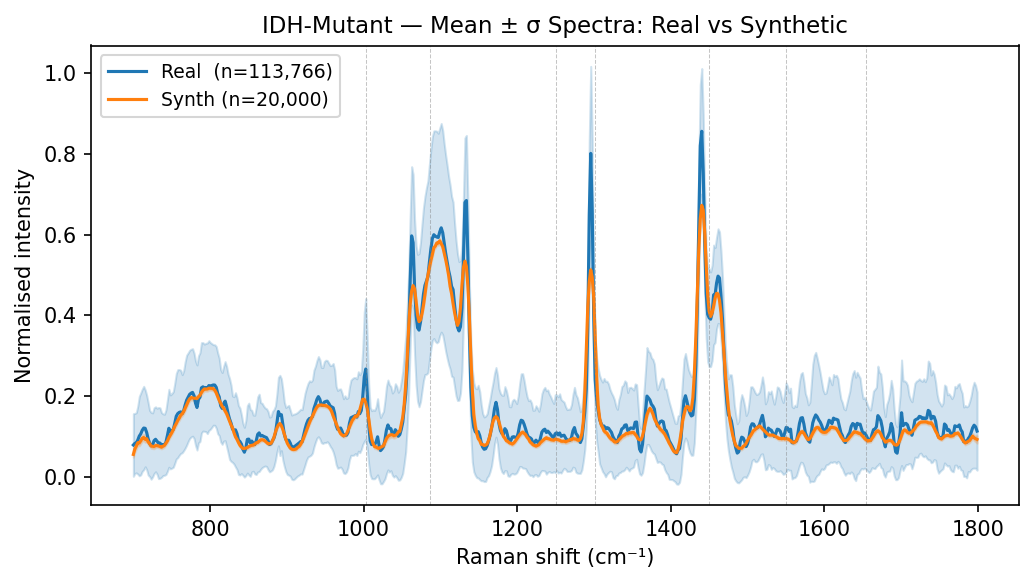
\includegraphics[width=0.85\textwidth]{images/A_mean_std_spectra_IDH-Mutant.png}
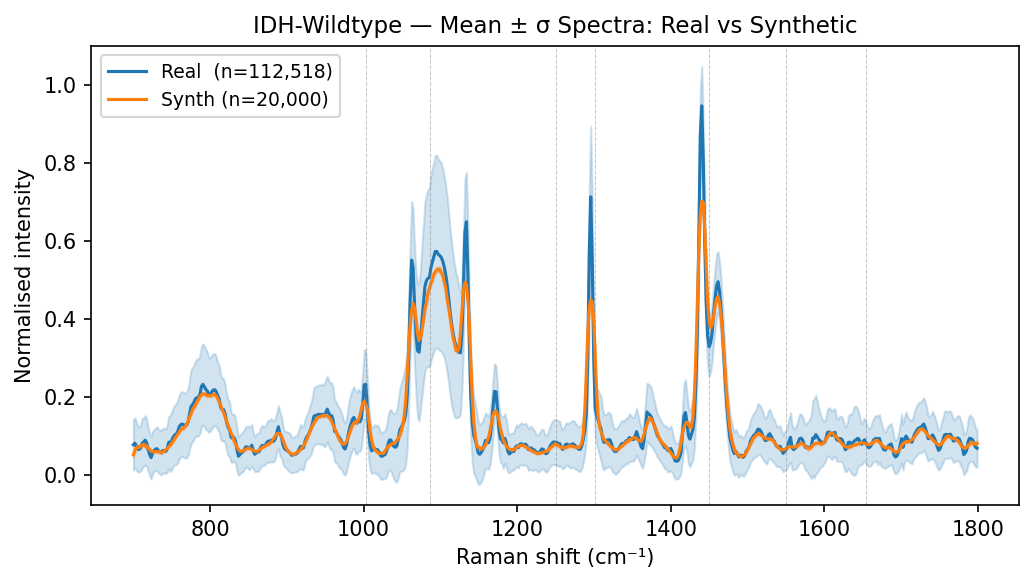
\includegraphics[width=0.85\textwidth]{images/A_mean_std_spectra_IDH-Wildtype.png}
\caption{Mean $\pm \sigma$ Raman spectra, real vs. synthetic, per class.}
\label{fig:mean_std_spectra}
\end{figure}

An important observation is that useful augmentation effects were obtained despite the relatively small number of independent patient samples available for training the generative model. In contrast to conventional deep generative modeling settings involving very large datasets, biomedical Raman spectroscopy typically operates in a data-constrained regime characterized by limited patient cohorts, acquisition variability, and strong intra-sample correlations. The present results indicate that generative models may still capture sufficient spectral structure to improve downstream robustness even when trained under these constraints.

The proposed Classification by Reconstruction (CbR) framework further demonstrates that the learned latent representations retain class-relevant spectral information. Although reconstruction-based inference did not outperform discriminative classifiers, its performance remained comparable to the TS/TR setting, suggesting that the generative model captures part of the discriminative structure of the underlying data distribution. More broadly, these results indicate that reconstruction-based inference may provide an alternative perspective for evaluating generative representations in biomedical spectroscopy.

\section{Limitations and Future Work}
\label{sec:limitations}

Several limitations remain. The dataset size is modest in terms of independent slide samples, and all experiments were conducted on a single acquisition setting. Moreover, the proposed spatio-spectral annotation pipeline includes heuristic and visually guided components that may introduce selection bias. The observed domain gap between synthetic and real spectra further indicates that the current CVAE architecture does not fully capture the variability present in the real data distribution, particularly for subtle multi-class grading tasks.

Future work could investigate larger multi-site datasets, alternative generative architectures such as diffusion-based models, and more systematic evaluation of synthetic spectrum fidelity and diversity. Additional directions include improving reconstruction-based inference strategies and exploring latent-space regularization methods better suited for highly heterogeneous biomedical spectral data.
